\documentclass[12pt,a4paper]{article}

% ─── Page Layout ───────────────────────────────────────────────────────────────
\usepackage[a4paper, margin=0.8in, headheight=14pt]{geometry}

% ─── Fonts (XeLaTeX) ───────────────────────────────────────────────────────────
\usepackage{fontspec}
\usepackage{unicode-math}
\setmainfont{TeX Gyre Pagella}
\setmonofont[Scale=0.88]{TeX Gyre Cursor}
\setmathfont{Latin Modern Math}

% ─── Packages ──────────────────────────────────────────────────────────────────
\usepackage{xcolor}
\usepackage{colortbl}
\usepackage{titlesec}
\usepackage{enumitem}
\usepackage{tabularx}
\usepackage{booktabs}
\usepackage{array}
\usepackage{amsmath}
\usepackage{tikz}
\usetikzlibrary{shapes.geometric, arrows.meta, positioning, calc, fit, decorations.pathreplacing}
\usepackage{tcolorbox}
\tcbuselibrary{skins, breakable}
\usepackage{hyperref}
\usepackage{fancyhdr}
\usepackage{graphicx}
\usepackage{microtype}
\hyphenpenalty=10000
\exhyphenpenalty=10000
\sloppy
\usepackage{caption}
\usepackage{setspace}
\usepackage{multirow}
\usepackage{tocloft}

% ─── Q&A helper ────────────────────────────────────────────────────────────────
\newcommand{\Q}[1]{\textbf{#1}\par\noindent\ignorespaces}

% ─── Colour Palette ────────────────────────────────────────────────────────────
\definecolor{myred}{RGB}{196,30,58}
\definecolor{mydark}{RGB}{30,30,50}
\definecolor{mygreen}{RGB}{14,120,80}
\definecolor{myteal}{RGB}{0,130,140}
\definecolor{myamber}{RGB}{180,100,0}
\definecolor{mypurple}{RGB}{100,30,160}
\definecolor{mygray}{RGB}{246,247,249}
\definecolor{mgframe}{RGB}{180,185,200}
\definecolor{watermark}{RGB}{145,150,170}
\definecolor{hdrred}{RGB}{250,232,235}
\definecolor{hdrgreen}{RGB}{220,244,233}
\definecolor{hdrteal}{RGB}{220,242,244}
\definecolor{hdramber}{RGB}{253,242,215}
\definecolor{hdrpurple}{RGB}{238,228,255}
\definecolor{hdrgray}{RGB}{238,240,245}
\definecolor{rowalt}{RGB}{250,251,253}

% ─── Section Formatting ────────────────────────────────────────────────────────
\titleformat{\section}
  {\large\bfseries\color{myred}}{\thesection.}{0.5em}{}
  [\vspace{1pt}{\color{myred}\rule{\linewidth}{0.8pt}}]
\titleformat{\subsection}
  {\normalsize\bfseries\color{myteal}}{\thesubsection}{0.5em}{}
\titlespacing*{\section}{0pt}{18pt}{7pt}
\titlespacing*{\subsection}{0pt}{11pt}{4pt}

% ─── Paragraph ─────────────────────────────────────────────────────────────────
\setlength{\parindent}{0pt}
\setlength{\parskip}{4pt}

% ─── TOC Styling ───────────────────────────────────────────────────────────────
\renewcommand{\cfttoctitlefont}{\large\bfseries\color{myred}}
\renewcommand{\cftaftertoctitle}{\par\noindent{\color{myred}\rule{\linewidth}{0.8pt}}}
\setlength{\cftbeforetoctitleskip}{0pt}
\setlength{\cftaftertoctitleskip}{6pt}
\renewcommand{\cftsecfont}{\normalsize\bfseries\color{mydark}}
\renewcommand{\cftsecpagefont}{\normalsize\bfseries\color{mydark}}
\renewcommand{\cftsecleader}{\cftdotfill{\cftdotsep}}
\setlength{\cftbeforesecskip}{7pt}
\renewcommand{\cftsubsecfont}{\small\color{mydark}}
\renewcommand{\cftsubsecpagefont}{\small\color{mydark}}
\setlength{\cftbeforesubsecskip}{3pt}
\setlength{\cftsubsecindent}{1.4em}

% ─── Table helpers ─────────────────────────────────────────────────────────────
\renewcommand{\arraystretch}{1.45}
\setlength{\tabcolsep}{6pt}
\arrayrulecolor{mydark}
\newcolumntype{B}[1]{>{\small\bfseries\raggedright\arraybackslash}m{#1}}
\newcolumntype{Y}{>{\small\raggedright\arraybackslash}X}
\renewcommand{\tabularxcolumn}[1]{m{#1}}

% ─── Header / Footer ───────────────────────────────────────────────────────────
\pagestyle{fancy}
\fancyhf{}
\fancyhead[L]{\small\color{myred}\textbf{PE-EC701A}\;\color{mydark}--- Microwave Theory and Technique}
\fancyhead[R]{\small\color{myteal}\textbf{Module 6 Notes}}
\fancyfoot[C]{\small\color{mydark}\thepage}
\fancyfoot[R]{\small\color{watermark}\textit{\copyright\ Biraj}}
\renewcommand{\headrulewidth}{0.5pt}
\renewcommand{\footrulewidth}{0.3pt}

% ─── Hyperref ──────────────────────────────────────────────────────────────────
\hypersetup{
  colorlinks=true, linkcolor=myteal, urlcolor=myteal,
  pdfauthor={Biraj Sarkar},
  pdftitle={PE-EC701A --- Module 6 Notes}
}

% ─── tcolorbox styles ──────────────────────────────────────────────────────────
\tcbset{
  tikzbox/.style={
    colback=mygray, colframe=mgframe, boxrule=0.6pt, arc=4pt,
    left=8pt, right=8pt, top=6pt, bottom=6pt,
    colbacktitle=mgframe, coltitle=mydark,
    fonttitle=\small\bfseries
  },
  defbox/.style={
    colback=hdrgreen, colframe=mygreen, boxrule=0.8pt, arc=4pt,
    left=9pt, right=9pt, top=6pt, bottom=6pt,
    colbacktitle=mygreen, coltitle=white,
    fonttitle=\small\bfseries
  },
  formulabox/.style={
    colback=hdrteal, colframe=myteal, boxrule=0.8pt, arc=4pt,
    left=9pt, right=9pt, top=7pt, bottom=7pt,
    colbacktitle=myteal, coltitle=white,
    fonttitle=\small\bfseries
  },
  examplebox/.style={
    colback=hdramber, colframe=myamber, boxrule=0.8pt, arc=4pt,
    left=9pt, right=9pt, top=6pt, bottom=6pt,
    colbacktitle=myamber, coltitle=white,
    fonttitle=\small\bfseries
  },
  masonbox/.style={
    colback=hdrpurple, colframe=mypurple, boxrule=0.8pt, arc=4pt,
    left=9pt, right=9pt, top=6pt, bottom=6pt,
    colbacktitle=mypurple, coltitle=white,
    fonttitle=\small\bfseries
  },
  exambox/.style={
    colback=hdrpurple, colframe=mypurple, boxrule=1pt, arc=5pt,
    left=10pt, right=10pt, top=8pt, bottom=8pt,
    colbacktitle=mypurple, coltitle=white,
    fonttitle=\bfseries,
    breakable, title after break={\textbf{Frequently Asked / Viva Questions (contd.)}}}
}
% Make all boxes breakable across pages
\tcbset{breakable}

% ─── TikZ styles ───────────────────────────────────────────────────────────────
\tikzset{
  block/.style={rectangle, draw=myteal, fill=hdrteal,
    text width=2.4cm, align=center, minimum height=0.95cm,
    font=\small, rounded corners=3pt, line width=0.7pt},
  redblock/.style={rectangle, draw=myred, fill=hdrred,
    text width=2.4cm, align=center, minimum height=0.95cm,
    font=\small, rounded corners=3pt, line width=0.7pt},
  netnode/.style={rectangle, draw=myteal, fill=hdrteal,
    text width=1.5cm, align=center, minimum height=0.8cm,
    font=\small, rounded corners=3pt, line width=0.7pt},
  sumjunc/.style={circle, draw=myamber, fill=hdramber,
    minimum size=0.62cm, font=\small, line width=0.8pt},
  snode/.style={circle, draw=mypurple, fill=hdrpurple,
    minimum size=0.55cm, font=\footnotesize, line width=0.7pt},
  arrow/.style={-Stealth, thick, color=mydark},
  redarrow/.style={-Stealth, thick, color=myred},
  line/.style={thick, color=mydark}
}

% ═══════════════════════════════════════════════════════════════════════════════
\begin{document}
% ═══════════════════════════════════════════════════════════════════════════════

\begin{center}
  {\LARGE\bfseries\color{myred} PE-EC701A --- Microwave Theory and Technique}\\[5pt]
  {\normalsize\color{mydark} Semester VII \quad$\bullet$\quad 3L:0T:0P \quad$\bullet$\quad 3 Credits}\\[3pt]
  {\normalsize\color{myteal}\textbf{Module 6 Exam Notes: Microwave Design Principles}}\\[3pt]
  {\small\color{mydark} CGEC \;$|$\; B.Tech ECE (2023--27) \;$|$\; \textit{Biraj Sarkar}}
\end{center}
\vspace{2pt}
\noindent{\color{myred}\rule{\linewidth}{1.5pt}}
\vspace{2pt}

\hypersetup{linkcolor=mydark}
\tableofcontents
\hypersetup{linkcolor=myteal}
\newpage

% ===============================================================================
\section{Impedance Transformation and Matching}
% ===============================================================================

Impedance matching is crucial to ensure maximum power transfer and prevent reflections in microwave networks.

\subsection{Smith Chart Coordinates}
The Smith Chart is a polar plot of the complex reflection coefficient ($\Gamma$), mapped to constant resistance ($r$) and constant reactance ($x$) circles:

\begin{tcolorbox}[tikzbox, title={Smith Chart Constant Circles Concept}]
\centering
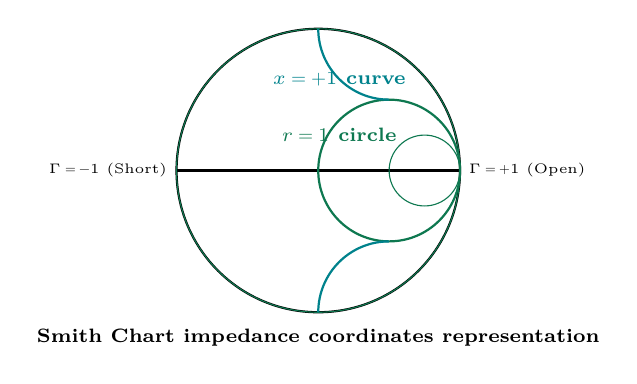
\begin{tikzpicture}[scale=0.9, every node/.style={font=\tiny}]
  % Outer boundary
  \draw[thick] (0,0) circle (2.0cm);
  
  % Real axis
  \draw[thick] (-2,0) -- (2,0);
  \node[left] at (-2,0) {$\Gamma = -1$ (Short)};
  \node[right] at (2,0) {$\Gamma = +1$ (Open)};
  
  % Constant Resistance circles (all touch (2,0))
  \draw[color=mygreen, thick] (1,0) circle (1.0cm); % r = 1
  \draw[color=mygreen, thin] (1.5,0) circle (0.5cm); % r = 3
  \draw[color=mygreen, thin] (0,0) circle (2.0cm); % r = 0 (same as boundary)
  
  % Constant Reactance curves
  % x = +1 curve
  \draw[color=myteal, thick] (1,1) arc (270:180:1.0cm);
  \draw[color=myteal, thick] (1,-1) arc (90:180:1.0cm);
  
  \node[color=mygreen, font=\scriptsize\bfseries] at (0.3,0.5) {$r=1$ circle};
  \node[color=myteal, font=\scriptsize\bfseries] at (0.3,1.3) {$x=+1$ curve};
  \node[below, font=\scriptsize\bfseries] at (0,-2.1) {Smith Chart impedance coordinates representation};
\end{tikzpicture}
\end{tcolorbox}

\subsection{Single-Stub Matching}
A single-stub tuner uses a shunt (or series) short- or open-circuited transmission line stub placed at a distance $d$ from the load to match a load impedance $Z_L$ to the line impedance $Z_0$.

\begin{tcolorbox}[tikzbox, title={Shunt Single-Stub Matching Network}]
\centering
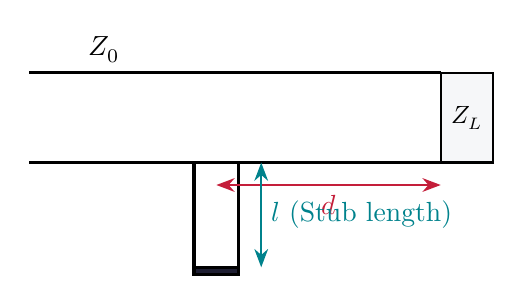
\begin{tikzpicture}[scale=0.95]
  % Main lines
  \draw[very thick] (0,0.6) -- (5.5,0.6);
  \draw[very thick] (0,-0.6) -- (5.5,-0.6);
  
  % Load box
  \draw[thick, fill=mygray] (5.5,-0.6) rectangle (6.2,0.6) node[midway, font=\small] {$Z_L$};
  
  % Shunt Stub (short-circuited at bottom)
  \draw[very thick] (2.2,-0.6) -- (2.2,-2.0);
  \draw[very thick] (2.8,-0.6) -- (2.8,-2.0);
  \draw[very thick, fill=mydark] (2.2,-2.0) rectangle (2.8,-2.1); % short circuit
  
  % Dimension arrows
  \draw[Stealth-Stealth, thick, color=myred] (2.5,-0.9) -- (5.5,-0.9) node[midway, below] {$d$};
  \draw[Stealth-Stealth, thick, color=myteal] (3.1,-0.6) -- (3.1,-2.0) node[midway, right] {$l$ (Stub length)};
  
  \node[above] at (1,0.6) {$Z_0$};
\end{tikzpicture}
\end{tcolorbox}

\subsubsection{Design Equations for Shunt Single-Stub}
Let $Y_L = 1/Z_L = G_L + j B_L$ be the load admittance. We normalize to $Y_0 = 1/Z_0$:
\begin{equation}
  y_L = g_L + j b_L = \frac{Y_L}{Y_0}
\end{equation}
The distance $d$ is chosen such that the admittance looking into the line at $d$ is:
\begin{equation}
  y_d = 1 + j b
\end{equation}
The stub length $l$ is then selected to provide a susceptance of $-j b$, canceling the reactive part and leaving a perfect match ($y_{\text{in}} = y_d + y_{\text{stub}} = 1$).
\begin{align}
  d &= \frac{\lambda}{2\pi} \tan^{-1}\left( \frac{r_L - 1}{x_L} \right) \quad (\text{simplified for specific cases}) \\
  l_s &= -\frac{\lambda}{2\pi} \tan^{-1}(b) \quad (\text{short-circuited stub})
\end{align}

% ===============================================================================
\section{Microwave Filter Design}
% ===============================================================================

Filters restrict frequencies allowed to pass. The modern \textbf{Insertion Loss Method} uses low-pass filter (LPF) prototypes with normalized values ($g_i$):
\begin{itemize}[leftmargin=*, itemsep=3pt]
  \item \textbf{Maximally Flat (Butterworth):} Flat passband response, roll-off is smooth.
  \item \textbf{Equal Ripple (Chebyshev):} Sharp cutoff, containing ripples in the passband.
\end{itemize}

\begin{tcolorbox}[formulabox, title={\textbf{Butterworth Prototype Values}}]
For a maximally flat low-pass filter, the element values $g_i$ ($1 \le i \le N$) are:
\begin{equation}
  g_i = 2 \sin \left[ \frac{(2i-1)\pi}{2N} \right] \quad \text{for } i = 1, 2, \dots, N
\end{equation}
And $g_{N+1} = 1.0$ for all $N$.
\end{tcolorbox}

% ===============================================================================
\section{RF and Microwave Amplifier Design}
% ===============================================================================

Microwave amplifier design utilizes active devices (transistors) characterized by their S-parameters:

\begin{tcolorbox}[tikzbox, title={Microwave Transistor Amplifier Block Diagram}]
\centering
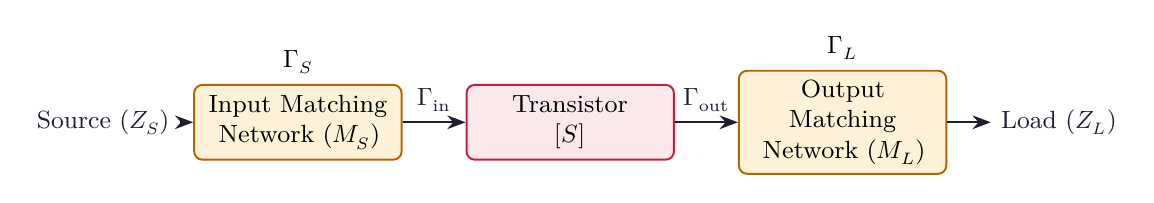
\begin{tikzpicture}[node distance=0.5cm and 0.8cm, every node/.style={font=\small}]
  \node[block, draw=myamber, fill=hdramber] (imn) {Input Matching\\Network ($M_S$)};
  \node[block, right=0.8cm of imn, draw=myred, fill=hdrred] (tx) {Transistor\\$[S]$};
  \node[block, right=0.8cm of tx, draw=myamber, fill=hdramber] (omn) {Output Matching\\Network ($M_L$)};
  
  \draw[arrow] (-1.5,0) node[left] {Source ($Z_S$)} -- (imn);
  \draw[arrow] (imn) -- (tx) node[midway, above] {$\Gamma_{\text{in}}$};
  \draw[arrow] (tx) -- (omn) node[midway, above] {$\Gamma_{\text{out}}$};
  \draw[arrow] (omn) -- (8.8,0) node[right] {Load ($Z_L$)};
  
  \node[above] at (imn.north) {$\Gamma_S$};
  \node[above] at (omn.north) {$\Gamma_L$};
\end{tikzpicture}
\end{tcolorbox}

\subsection{Amplifier Stability Criteria}
An amplifier is \textbf{unconditionally stable} if the transistor will not oscillate for any passive source and load impedance ($\text{Re}(Z_S), \text{Re}(Z_L) > 0$).
This requires the Rollett stability factor ($K$) to exceed 1 and the matrix determinant delta ($|\Delta|$) to be less than 1:

\begin{tcolorbox}[formulabox, title={\textbf{Rollett Stability Criteria}}]
\begin{align}
  K &= \frac{1 - |S_{11}|^2 - |S_{22}|^2 + |\Delta|^2}{2 |S_{12} S_{21}|} > 1 \\
  |\Delta| &= |S_{11}S_{22} - S_{12}S_{21}| < 1
\end{align}
If $K < 1$, the amplifier is only \textbf{conditionally stable}, and matching networks ($\Gamma_S, \Gamma_L$) must be chosen outside the unstable regions defined by the \textbf{stability circles}.
\end{tcolorbox}

\subsection{Amplifier Power Gains}
\begin{itemize}[leftmargin=*, itemsep=3pt]
  \item \textbf{Transducer Power Gain ($G_T$):} The ratio of power delivered to the load to the power available from the source.
    \begin{equation}
      G_T = \frac{1 - |\Gamma_S|^2}{|1 - S_{11}\Gamma_S|^2} |S_{21}|^2 \frac{1 - |\Gamma_L|^2}{|1 - S_{22}\Gamma_L - \frac{S_{12}S_{21}\Gamma_S\Gamma_L}{1 - S_{11}\Gamma_S}|^2}
    \end{equation}
  \item \textbf{Unilateral Transducer Gain ($G_{TU}$):} Assumes negligible feedback ($S_{12} = 0$).
    \begin{equation}
      G_{TU} = \frac{1 - |\Gamma_S|^2}{|1 - S_{11}\Gamma_S|^2} |S_{21}|^2 \frac{1 - |\Gamma_L|^2}{|1 - S_{22}\Gamma_L|^2}
    \end{equation}
\end{itemize}

\subsection{Low Noise Amplifier (LNA) Design \& Noise Figure Circles}
In LNA design (critical for receiver front-ends), the goal is to achieve the lowest possible Noise Figure ($F$), even at the expense of maximum transducer gain.
\begin{itemize}[leftmargin=*, itemsep=3pt]
  \item \textbf{Noise Figure Formula:}
    \begin{equation}
      F = F_{\text{min}} + \frac{4 R_n}{Z_0} \frac{|\Gamma_S - \Gamma_{\text{opt}}|^2}{(1 - |\Gamma_S|^2) |1 + \Gamma_{\text{opt}}|^2}
    \end{equation}
    where $F_{\text{min}}$ is the minimum noise figure of the transistor, $R_n$ is the equivalent noise resistance, $\Gamma_{\text{opt}}$ is the optimum source reflection coefficient, and $\Gamma_S$ is the actual source reflection coefficient.
  \item \textbf{Noise Figure Circles:} For a target noise figure $F > F_{\text{min}}$, the locus of all source reflection coefficients $\Gamma_S$ forms a circle on the Smith Chart.
    \begin{itemize}[leftmargin=*, itemsep=2.5pt, topsep=0pt]
      \item \textbf{Center ($C_F$):}
        \begin{equation}
          C_F = \frac{\Gamma_{\text{opt}}}{1 + N}
        \end{equation}
      \item \textbf{Radius ($R_F$):}
        \begin{equation}
          R_F = \frac{\sqrt{N^2 + N(1 - |\Gamma_{\text{opt}}|^2)}}{1 + N}
        \end{equation}
      \item \textbf{Noise Parameter ($N$):}
        \begin{equation}
          N = \frac{F - F_{\text{min}}}{4 R_n/Z_0} |1 + \Gamma_{\text{opt}}|^2
        \end{equation}
    \end{itemize}
    The designer selects a source reflection coefficient $\Gamma_S$ lying on the desired Noise Figure circle that offers a reasonable trade-off with input matching and gain.
\end{itemize}

% ===============================================================================
\section{Microwave Mixer Design}
% ===============================================================================

Mixers are 3-port non-linear devices that perform frequency translation by multiplying the RF input signal ($f_{\text{RF}}$) with a Local Oscillator signal ($f_{\text{LO}}$), producing an Intermediate Frequency ($f_{\text{IF}} = |f_{\text{RF}} \pm f_{\text{LO}}|$).
\begin{itemize}[leftmargin=*, itemsep=3pt]
  \item \textbf{Single-Ended Diode Mixer:} Uses a single Schottky diode. It is simple but provides poor isolation between the RF and LO ports, and does not suppress LO amplitude noise.
  \item \textbf{Balanced Mixer:} Utilizes two Schottky diodes combined via a 3 dB hybrid junction (such as a Magic Tee or branch-line coupler).
  \begin{itemize}[leftmargin=*, itemsep=2.5pt, topsep=0pt]
    \item \textbf{LO Noise Suppression:} The hybrid junction feeds the LO signal to the two diodes out-of-phase ($180^\circ$) while feeding the RF signal in-phase. The combined output at the IF port cancels out the LO amplitude noise.
    \item \textbf{Isolation:} Provides high isolation ($>20\,\text{dB}$) between the RF and LO ports, preventing local oscillator power leakage back into the antenna.
  \end{itemize}
  \item \textbf{Conversion Loss ($L_C$):} The ratio of RF input power to the desired IF output power:
    \begin{equation}
      L_C = 10 \log_{10}\left( \frac{P_{\text{RF}}}{P_{\text{IF}}} \right) \quad (\text{dB})
    \end{equation}
    For passive diode mixers, typical conversion loss ranges from $5\,\text{dB}$ to $8\,\text{dB}$.
\end{itemize}

% ===============================================================================
\section{Microwave Oscillator Design}
% ===============================================================================

Microwave oscillators convert DC power into RF power using active devices (transistors with positive feedback, or negative resistance diodes like Gunn and IMPATT).

\subsection{One-Port Negative Resistance Oscillator}
An active device presenting a negative input impedance $Z_{\text{in}} = R_{\text{in}} + j X_{\text{in}}$ (where $R_{\text{in}} < 0$) is terminated with a passive load impedance $Z_L = R_L + j X_L$:
\begin{itemize}[leftmargin=*, itemsep=3pt]
  \item \textbf{Startup Condition:} For oscillations to initiate from thermal noise:
    \begin{equation}
      R_{\text{in}} + R_L < 0 \quad \text{and} \quad X_{\text{in}} + X_L = 0
    \end{equation}
  \item \textbf{Steady-State Stability:} As the oscillation amplitude $A$ builds up, the negative resistance $R_{\text{in}}(A)$ saturates (becomes less negative) due to device non-linearities until a stable operating amplitude $A_0$ is reached:
    \begin{equation}
      R_{\text{in}}(A_0) + R_L = 0 \quad \text{and} \quad X_{\text{in}}(A_0) + X_L = 0
    \end{equation}
\end{itemize}

\subsection{Two-Port Transistor Oscillator}
A transistor-based oscillator uses an active three-terminal device (e.g., GaAs MESFET). An unstable termination at one port (such as a capacitive load at the source) is used to generate a negative input resistance at the other port (gate), which is then connected to a high-$Q$ resonant circuit (tuning network) to establish oscillation at the desired frequency.

\subsection{Microwave Power Amplifier Design}
Microwave power amplifiers (PAs) are designed to deliver high RF power levels to a load (typically a transmitting antenna) with maximum efficiency and minimal distortion.
\begin{itemize}[leftmargin=*, itemsep=3pt]
  \item \textbf{1-dB Compression Point ($P_{1\text{dB}}$):} As input power increases, the amplifier eventually saturates and gain drops. The $P_{1\text{dB}}$ is the power level at which the output power is $1\text{ dB}$ lower than it would be in the ideal linear region. It marks the boundary of the linear operating region.
  \item \textbf{Power Added Efficiency (PAE):} A critical metric for PAs that accounts for the input RF power, expressing the net RF power generated relative to the DC power consumed:
    \begin{equation}
      \text{PAE} = \frac{P_{\text{RF, out}} - P_{\text{RF, in}}}{P_{\text{DC}}} \times 100\%
    \end{equation}
  \item \textbf{Drain/Collector Efficiency ($\eta$):} Ratio of output RF power to input DC power: $\eta = P_{\text{RF, out}}/P_{\text{DC}} \times 100\%$.
\end{itemize}

\textbf{Power Amplifier Classes:}\par\noindent
PAs are classified based on their conduction angle ($\theta_c$), which defines the fraction of the RF cycle during which the active transistor conducts current.
\par\noindent
{\renewcommand{\arraystretch}{1.65}%
\begin{tabularx}{\linewidth}{|B{1.6cm}|Y|Y|Y|Y|}\hline
\textbf{Class} & \textbf{Conduction Angle ($\theta_c$)} & \textbf{Ideal Max Efficiency} & \textbf{Linearity} & \textbf{Characteristics} \\[4pt]
\hline
Class A & $360^\circ$ (conducts full cycle) & $50\%$ & Outstanding & Low efficiency; high heat dissipation; active at all times. \\[4pt]
\hline
Class AB & $180^\circ < \theta_c < 360^\circ$ & $50\% - 78.5\%$ & Good & Compromise between Class A and B; commonly used in RF links. \\[4pt]
\hline
Class B & $180^\circ$ (conducts half cycle) & $78.5\%$ & Moderate & Transistor conducts only during one half-cycle; requires push-pull. \\[4pt]
\hline
Class C & $<180^\circ$ (conducts narrow pulses) & $>85\%$ (approaching $100\%$) & Very Poor & High distortion; requires resonant tank circuit to reconstruct wave. \\[4pt]
\hline
\end{tabularx}
}

\begin{center}
  {\large\bfseries\color{myred} Quick Revision --- Module VI}\\[3pt]
  {\small\color{mydark} Microwave Design Principles $|$ PE-EC701A}
\end{center}
\noindent{\color{myred}\rule{\linewidth}{1.2pt}}
\vspace{4pt}

\begin{tcolorbox}[formulabox, title={\textbf{Key Formulas at a Glance}}]
\renewcommand{\arraystretch}{1.3}
\begin{tabularx}{\linewidth}{B{4.5cm} X}Rollett Stability factor & $K = \frac{1 - |S_{11}|^2 - |S_{22}|^2 + |\Delta|^2}{2|S_{12}S_{21}|}$ \\[4pt]
Determinant delta       & $\Delta = S_{11}S_{22} - S_{12}S_{21}$ \\[4pt]
Unilateral gain         & $G_{TU} = \frac{1-|\Gamma_S|^2}{|1-S_{11}\Gamma_S|^2} |S_{21}|^2 \frac{1-|\Gamma_L|^2}{|1-S_{22}\Gamma_L|^2}$ \\[4pt]
Butterworth filter      & $g_i = 2 \sin\left(\frac{(2i-1)\pi}{2N}\right)$ \\[4pt]
Unilateral figure merit  & $U = \frac{|S_{11}S_{12}S_{21}S_{22}|}{(1-|S_{11}|^2)(1-|S_{22}|^2)}$ \\[4pt]
LNA Noise Parameter ($N$) & $N = \frac{F - F_{\text{min}}}{4 R_n/Z_0} |1 + \Gamma_{\text{opt}}|^2$ \\[4pt]
LNA Circle Center ($C_F$) & $C_F = \frac{\Gamma_{\text{opt}}}{1 + N}$ \\[4pt]
LNA Circle Radius ($R_F$) & $R_F = \frac{\sqrt{N^2 + N(1 - |\Gamma_{\text{opt}}|^2)}}{1 + N}$
\end{tabularx}
\tcbset{colbacktitle=mygreen, coltitle=white}
\end{tcolorbox}

\begin{tcolorbox}[defbox, title={\textbf{One-Line Definitions}}]
\begin{itemize}[leftmargin=*, itemsep=2.5pt, topsep=0pt]
  \item \textbf{Smith Chart:} A graphical utility mapping reflection coefficients to complex impedances.
  \item \textbf{Stub Tuning:} Impedance matching using shunt or series transmission line segments.
  \item \textbf{Butterworth Filter:} A filter designed for a maximally flat amplitude response in the passband.
  \item \textbf{Chebyshev Filter:} A filter that provides sharp roll-off at the expense of equal-ripple passband ripples.
  \item \textbf{Rollett Stability:} Mathematical check ($K > 1$) determining if an amplifier is unconditionally stable.
  \item \textbf{LNA:} Low Noise Amplifier, designed to minimize noise figure circles on the input matching network.
  \item \textbf{Stability Circles:} Regions plotted on the Smith Chart enclosing unstable source/load reflection coefficients.
  \item \textbf{Conversion Loss:} The ratio of RF input power to IF output power in a passive mixer (expressed in dB).
  \item \textbf{Balanced Mixer:} A mixer using a hybrid junction to combine two diodes, canceling LO noise and providing port isolation.
  \item \textbf{One-Port Oscillator:} An oscillator designed by terminating a negative-resistance device with a resonant load.
\end{itemize}
\end{tcolorbox}

\begin{tcolorbox}[exambox, title={\textbf{Frequently Asked / Viva Questions}}]
\begin{enumerate}[topsep=0pt, label=\textbf{Q\arabic*.}, itemsep=5pt]
  \item \Q{What are constant resistance and constant reactance circles on a Smith Chart?}
    Constant resistance circles are circles whose centers lie on the horizontal real axis, all passing through the open-circuit point. Constant reactance circles are arcs representing imaginary parts.
  \item \Q{What is the difference between single-stub and double-stub matching?}
    Single-stub matching requires adjusting both the stub length and its position from the load. Double-stub matching uses fixed-position stubs, adjusting only their lengths.
  \item \Q{State the conditions for unconditional stability in microwave amplifiers.}
    The Rollett stability factor $K$ must be greater than 1 ($K > 1$) and the S-parameter determinant magnitude $|\Delta|$ must be less than 1 ($|\Delta| < 1$).
  \item \Q{Why are short-circuited stubs preferred over open-circuited stubs?}
    Because open-circuited stubs radiate energy from their open ends, behaving as antennas. Short-circuited stubs confine fields and are easier to manufacture with high precision.
  \item \Q{What is the unilateral assumption in amplifier design?}
    The assumption that $S_{12} = 0$, meaning there is no feedback from output to input. This simplifies the design of matching networks.
  \item \Q{Explain the insertion loss method of filter design.}
    It designs filters based on a power transfer function (like Butterworth or Chebyshev), yielding element values ($g_i$) normalized to a $1\,\Omega$ source and $1$ rad/s cutoff.
  \item \Q{What is the significance of Noise Figure Circles in LNA design?}
    They map the source reflection coefficients ($\Gamma_S$) that produce a constant noise figure, allowing the designer to balance noise figure and gain.
  \item \Q{Under what condition is single-stub matching not possible?}
    When the load impedance lies within a specific prohibited region of the Smith Chart (for a given shunt or series configuration), requiring a different stub location.
  \item \Q{What are Richards' Transformations?}
    Mathematical maps that convert lumped inductors and capacitors into transmission line stubs ($\text{L} \to \text{short stub}$, $\text{C} \to \text{open stub}$) at microwave frequencies.
  \item \Q{What is Kuroda's Identity?}
    A set of network equivalence rules used to separate filter stubs using redundant transmission line sections (unit elements).
  \item \Q{Explain the difference between power gain, available gain, and transducer gain.}
    Transducer gain accounts for mismatch at both input and output. Available gain assumes matched output. Power gain assumes matched input.
  \item \Q{What is the Unilateral Figure of Merit ($U$)?}
    A ratio used to calculate the maximum error introduced when assuming $S_{12} = 0$ instead of using the bilateral gain equations.
  \item \Q{State the startup and steady-state conditions for a negative resistance one-port oscillator.}
    Startup: $R_{\text{in}} + R_L < 0$ and $X_{\text{in}} + X_L = 0$ (net loop resistance is negative, allowing oscillations to build from thermal noise). Steady-state: $R_{\text{in}}(A_0) + R_L = 0$ and $X_{\text{in}}(A_0) + X_L = 0$ (saturation reduces negative resistance until net loop resistance is zero, sustaining a stable amplitude $A_0$).
  \item \Q{How does a balanced mixer achieve LO noise suppression?}
    By using a 3 dB hybrid junction (such as a Magic Tee) that feeds the local oscillator (LO) signal to the two diodes $180^\circ$ out-of-phase, while feeding the RF signal in-phase. The combined IF output cancels the LO amplitude noise components.
\end{enumerate}
\tcbset{colbacktitle=mgframe, coltitle=mydark}
\end{tcolorbox}

\begin{tcolorbox}[tikzbox, title={Comparison of Single-Stub and Double-Stub Tuning}]
\renewcommand{\arraystretch}{1.4}
\par\noindent
{\renewcommand{\arraystretch}{1.55}%
\begin{tabularx}{\linewidth}{|B{3.2cm}|Y|Y|}\hline
\textbf{Feature} & \textbf{\color{myteal}Single-Stub Tuning} & \textbf{\color{myamber}Double-Stub Tuning} \\[4pt]
\hline
\textbf{Stub Position} & Must be variable (requires sliding stub or custom line length). & Fixed spacing (typically $\lambda/8$ or $3\lambda/8$). \\[4pt]
\hline
\textbf{Adjustment} & Adjusts both stub length and stub distance from the load. & Adjusts only the lengths of the two stubs. \\[4pt]
\hline
\textbf{Matching Range} & Can match any load impedance with non-zero real part. & Cannot match all loads (contains a "forbidden region"). \\[4pt]
\hline
\textbf{Implementation} & Difficult in microstrip (requires changing physical layout). & Easy in microstrip (stubs are printed at fixed locations). \\[4pt]
\hline
\end{tabularx}
}
\end{tcolorbox}

\end{document}
